\documentclass{article}
\usepackage[utf8]{inputenc}
\usepackage{amsmath}
\usepackage{cancel}
\usepackage{graphicx}

\title{Continuación sección 3.3 página 102}
\author{Angel Luis Robles Fernandez}
\date{June 2020}

\begin{document}

\maketitle

\section{Sección 3.37}
El potencial está dado como:
\begin{equation}
    \Phi(Z = r) = \sum_{l = 0}^{\infty} [A_l \gamma^l + B_l \gamma^{-(l+1)}]
\end{equation}
Una importante expansión es que el potencial en $\vec{x}$ debido a una carga puntual en el punto $\vec{x \prime}$

\begin{figure}[h]-
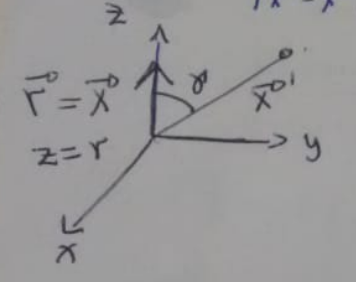
\includegraphics[width=4cm]{image1.png}
\centering
\end{figure}


\begin{equation}
    \frac{1}{|\vec{x} - \vec{x \prime} |} = \sum_{l}^{\infty}  (A_l \gamma^l + B_l \gamma^-{-(l+1)})P_l(\cos \gamma)  
\end{equation}

\begin{equation}
\begin{gathered}
    \vec{x\prime} =  r\prime \cos \varphi \prime \sin \theta \prime r\prime \sin \varphi \prime \sin \theta\prime + r\prime \cos \theta \prime \\
    \vec{x} = \vec{r} \\
    \vec{x} - \vec{x \prime} = (x - x\prime)\hat{i} + (y - y\prime) \hat{j} + (z-z\prime)\hat{k} \\
    = -r\prime \cos \varphi \prime \sin \theta\prime \hat{i} - r\prime \sin \varphi \prime \sin \theta \prime + (z - r\prime \cos \theta \prime)
\end{gathered}
\end{equation}

\begin{equation}
    \begin{gathered}
        |\vec{x} - \vec{x\prime}| ^2 = r \prime ^2 \cos ^2 \varphi \prime \sin ^2\theta \prime + r\prime ^2 \sin ^2 \varphi \prime \sin ^2 \theta\prime + \\ 
    (z -r \prime \cos \theta \prime)^{2} \\
    = r^2\prime (\cos^2 \varphi \prime + \sin^2\varphi \prime) \sin ^2 \theta \prime + (z - r\prime \cos \theta \prime)^2 \\
    = r \prime ^2 \sin ^2 \theta \prime + z^2 - 2zr\prime \cos \theta \prime + r \prime ^2 \cos ^2 \theta \prime \\
    = r\prime ^2 + z^2 - 2 z r \prime \cos \theta \prime
        \end{gathered}
\end{equation}

donde $z = r$ con  $\theta \prime = \gamma$

\begin{equation}
    \begin{gathered}
    |\vec{x}- \vec{x\prime}|^2 = r\prime ^2 + r^2 - 2r r\prime \cos \theta \prime \\
    |\vec{x} - \vec{x\prime}| = (r^2\prime + r^2 - 2 r r\prime \cos \gamma)^{1/2}
    \end{gathered}
\end{equation}


\begin{figure}[h]
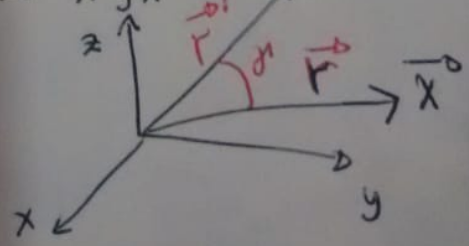
\includegraphics[width=4cm]{image2}
\centering
\end{figure}

donde: \\
$r_<$ es el más pequeño entre $|\vec{x}|$ y $|\vec{x\prime}|$ \\
$r_>$ es el más grande entre $|\vec{x}|$ y $|\vec{x\prime}|$ \\
$\gamma$ es el ángulo entre $\vec{x}$ y $\vec{x\prime}$

donde factorizando $r\prime$

\begin{equation}
    \begin{gathered}
    |\vec{x} - \vec{x\prime}| = (r^2\prime + r^2 - 2 r r\prime \cos \gamma)^{1/2} \\
    = \left [ r^2\prime \left( 1 + \frac{r^2}{r^2\prime} - 2 r \frac{ r \prime }{r^{2}\prime} \cos \gamma \right) \right] \\
    = r\prime \left (1 + \left (\frac{r}{r\prime}\right )^2 - 2 \frac{r}{r\prime}\cos\gamma \right)
\end{gathered}
\end{equation}

con $r < r\prime$, factorizando $r^2$
\begin{equation}
    \begin{gathered}
    |\vec{x} - \vec{x\prime}| = r \left ( 1 + \left (\frac{r\prime}{r} \right )^2 - 2 \frac{r\prime}{r}\cos \gamma \right )^{1/2} \\
    \frac{1}{|\vec{x} - \vec{x\prime}|} = \frac{1}{ r \left [ 1 + \left (\frac{r\prime}{r} \right )^2 - 2 \frac{r\prime}{r}\cos \gamma \right ]^{1/2}  }
    \end{gathered}
\end{equation}

\begin{equation}
     \frac{1}{|\vec{x} - \vec{x\prime}|} = \frac{1}{r} \sum_{l = 0}{\infty}P_l(\cos \gamma) \left( \frac{r\prime}{r} \right)^l
\end{equation}

\begin{equation}
 \frac{1}{|\vec{x} - \vec{x\prime}|} = \sum_{l=0}^{\infty} P_l(\cos\gamma) \frac{ (r\prime)^l}{r^{l+1}}    
\end{equation}

Regresando a la primera ecuación del grupo:

\begin{equation}
    \begin{gathered}
    \frac{1}{|\vec{x} - \vec{x\prime}|} = \frac{1}{r\prime \left(1 + \left( \frac{r}{r\prime} \right)^2 - 2 \left (\frac{r}{r\prime} \right )\cos \gamma \right)^{1/2} } \\
    = \frac{1}{r\prime} \sum_{l = 0}^{\infty} P_{l}(\cos \gamma) \left( \frac{r}{r\prime} \right )^l
    =     \frac{1}{|\vec{x} - \vec{x\prime}|} = \sum_{l = 0 }^{\infty} P_l(\cos \gamma) \frac{r^l}{(r\prime)^{l+1}}
    \end{gathered} 
\end{equation}
Para $r < r\prime$
En general se tiene que:
\begin{equation}
    \label{eq:3.38}
    \frac{1}{|\vec{x}-\vec{x\prime}|} = \sum_{l = 0}^{\infty} P_l(\cos \gamma) \frac{(r_<)^l}{(r_>)^{l+1}}
\end{equation}
para puntos fuera del eje $z$

Otro ejemplo es el potencial debido a una carga total $q$ uniformemente bien distribuída al rededor de un anillo circular del radio $a$, como se muestra en la figura (3.4), donde el centro del anillo está sobre el eje $z$ a la altura de $z = b$. El potencial en el punto $P$ sobre el eje de simetría con $z = r$ es $\frac{q}{4\pi \varepsilon_0}$ dividido entre la distancia $AP$


\begin{figure}[h]
\centering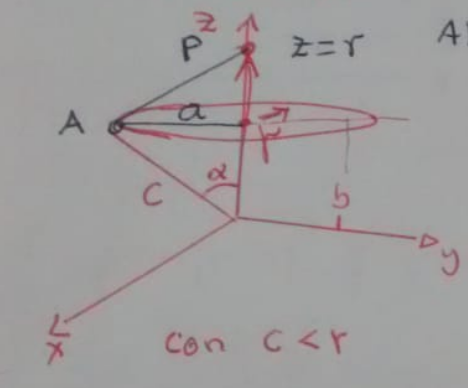
\includegraphics[width=4cm]{image3.png}
\caption{Figura 3.4}
\end{figure}

\begin{equation}
    AP = (r^2 + c^2 - 2rc\cos \gamma)^{1/2}
\end{equation}
\begin{equation}
    \Phi(z=r) = \frac{1}{4\pi \varepsilon_0 (r^2 + c^2 - 2rc\cos \gamma)^{1/2}}
\end{equation}
\begin{equation}
    \begin{gathered}
    c^2 = a^2 + b^2 \\
    \tan \alpha = \frac{a}{b}\\
    \alpha = \arctan \left( \frac{a}{b}\right )
    \end{gathered}
\end{equation}

\begin{equation}
    \begin{gathered}
    (r^2 + c^2 - 2rc\cos\gamma)^{1/2} = \left [r^2(1 + \left(\frac{c}{r}\right)^2 - \frac{2{r}c}{r^{2}} \cos \gamma ) \right]^{1/2} \\
    = r (1 + \left(\frac{c}{r} \right )^2 - 2 \frac{c}{r}\cos\gamma )^{1/2}
    \end{gathered}
\end{equation}

\begin{equation}
    \Phi(z = r) = \frac{q}{4\pi\varepsilon_0} \frac{1}{ r (1 + \left(\frac{c}{r} \right )^2 - 2 \frac{c}{r}\cos\gamma )^{1/2} }
\end{equation}

para $r > c$
\begin{equation}
    \Phi(z = r) = \frac{q}{4\pi\varepsilon_0} \frac{1}{r} \sum_l P_l \left(\cos \gamma) \frac{c}{\gamma}\right)^l 
\end{equation}
lejos del anillo:

\begin{equation}
    \Phi(z = r) = \frac{q}{4\pi\varepsilon_0} \frac{1}{r} \sum_l P_l \left(\cos \gamma) \frac{c^l}{\gamma^{l+1}}\right)^l 
\end{equation}
para $c > r$

\begin{equation}
    \Phi(z = r) = \frac{q}{4\pi\varepsilon_0} \frac{1}{r} \sum_l P_l \left(\cos \gamma) \frac{r}{c}\right)^l 
\end{equation}

y cuando el anillo es más grande (estoy cerca del anillo)


\begin{equation}
    \Phi(z = r) = \frac{q}{4\pi\varepsilon_0} \frac{1}{r} \sum_l P_l \left(\cos \gamma) \frac{r^l}{c^{l+2}}\right) 
\end{equation}

Para obtener el potencial en cualquier punto del espacio, se obtiene multiplicando cada miembro de esa serie por $P_l(\cos \theta)$ con $\gamma = \alpha$:
\begin{equation}
    \Phi(r, \theta) = \frac{q}{4 \pi \varepsilon_0} \sum_{l = 0}^{\infty} \frac{r_<^{l}}{r_>^{l + 1}} P_l(\cos \alpha) P_l(\cos \gamma)
\end{equation}

\section*{3.6 Teorema de adición para armónicos esféricos}
Considere dos vectores $\vec{x}$ y $\vec{x\prime}$ en coordenadas esféricas $(r, \theta,\varphi)$ y $(r\prime, \theta\prime,\varphi\prime)$ respectivamente, formando un ángulo $\gamma$ entre ellos. El teorema de adición expresa un polinomio de Legendre de orden $l$ en el ángulo $\gamma$ en términos de producto de armónicos esféricos de los ángulos $\theta,\varphi, \theta\prime \varphi\prime$

\begin{figure}[h]
\centering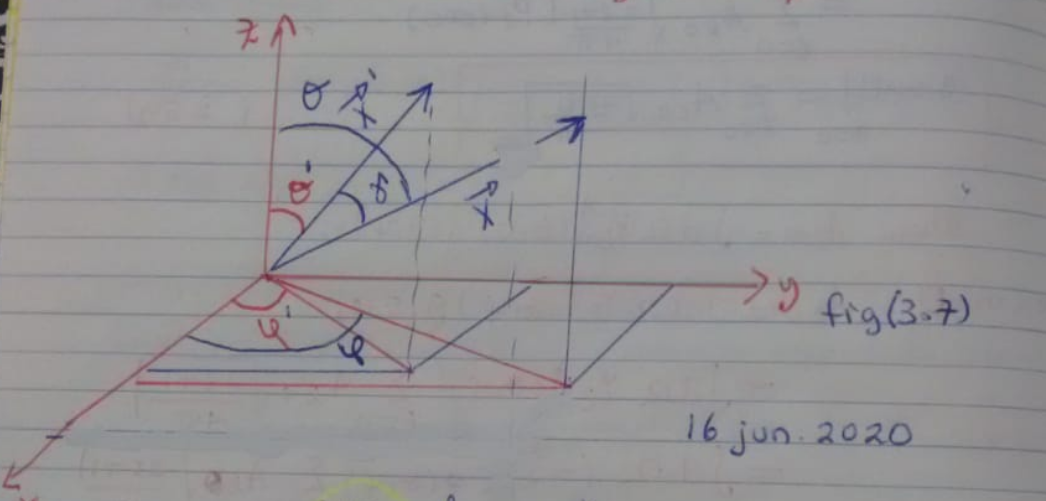
\includegraphics[width=4cm]{image4.png}
\caption{Figura 3.7}
\end{figure}


\begin{equation}
    P_l (\cos \gamma) = \frac{4\pi}{2l + 1} \sum_{m = -l}^{l} Y_{lm}^{*}(\theta\prime, \varphi\prime)Y_{lm}(\theta, \varphi)
\end{equation}

Utilizando:
\begin{equation}
    \begin{gathered}
    \cos (a\pmb) = \cos a \cos b \mp \sin a \sin b \\
    \cos \gamma = \cos\theta \cos \theta\prime + \sin \theta \sin \theta\prime \cos (\varphi - \varphi \prime)
    \end{gathered}
\end{equation}
Para probar el teorema consideramos que el vector $\vec{x\prime}$ est+a fijo en el espacio. Entonces $P_l ( \cos \gamma)$ es función de los ángulos $\theta$ y $\varphi$ siendo $\theta\prime$ y $\varphi\prime$ parámetros. Tenemos que una función arbitraria $g(\theta, \varphi)$ puede ser expandida en armónicos esféricos:
\begin{equation}
    g(\theta, \varphi) = \sum_{l = 0}^{\infty} \sum_{m = -l}^{l} A_{lm}Y_{lm}(\theta , \varphi)
\end{equation}
donde:
\begin{equation}
    A_{lm} = \int d\Omega Y_{lm}^{*}(\theta, \varphi) g(\theta, \varphi)
\end{equation}

\begin{equation}
P_l(\cos \gamma) = \sum_{l\prime = 0}^{\infty} \sum_{m = -l\prim}^{l\prime}A_{l\prime m}(\theta \prime, \varphi\prime) Y_{l\prime m} (\theta, \varphi)    
\end{equation}
donde comparando con 3.62 sólo aparecen términos con $l\prime = l$.  Para ver por qué esto es así vamos a colocar el sistema de coordenadas de tal manera que $\vec{x\prime}$ corresponde al eje $z$ y encones $\gamma$ es el ángulo polar $\gamma = \theta$


\begin{figure}[h]
\centering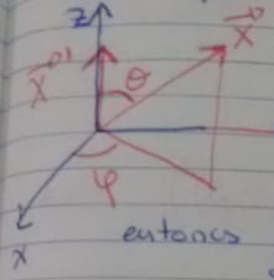
\includegraphics[width=4cm]{image5.png}
\caption{Figura 3.7 de la Eq. 3.63}
\end{figure}
entonces:
\begin{equation}
    \frac{d}{dx} \left ( (1-x^2) \frac{dP}{dx} \right ) + \left [ l(l+1) - \frac{m^2}{1-x^2}\right] P = 0
\end{equation}
Si $m = 0$:
\begin{equation}
\begin{gathered}
    \frac{d}{dx} (1 - x^2) \frac{dP}{dx} + (1 - x^2) \frac{d^2P}{dx^2} + l (l+1)P = 0 \\
    -2x\frac{dP}{dx} + (1 - x^2) \frac{d^2 P}{d x^2} + l(l+1)P=0
\end{gathered}
\end{equation}
Esto debe satisfacer la ecuación:
\begin{equation}
    \nabla^2 \prime P_l (\cos \gamma)+ \frac{l +(l+1)}{r^2} P_l(\cos \theta) = 0
\end{equation}
donde $\nabla^2 \prime$ es el laplaciano que se refiere a esos nuevos ejes. Si los ejes se restan a la posición de la figura 3.7 $\nabla^2 = \nabla ^2 \prime$ y $r$ no cambia. Consecuentemente $P_l(\cos \gamma)$ satisface la ec. (3.64)

Esto es armónicos esféricos de orden $l$. Esto significa que la combinación lineal de $Y_{lm}$
\begin{equation}
    P_l (\cos \gamma) = \sum_{m = -l}^{l} A_{m}(\theta\prime, \varphi\prime) Y_{lm}(\theta, \varphi)
\end{equation}

\begin{equation}
    P_l (\cos \gamma) = \sum_{m = -l}^{l} A_{ml} (\theta\prime, \varphi \prime)Y_{lm}(\tehta \varphi)
\end{equation}
donde:
\begin{equation}
    A_{lm} = \int d\Omega Y_{lm}^{*}(\theta , \varphi)g(\theta, \varphi)
\end{equation}
con $m = 0$ el coeficiente $\left (\frac{4\pi}{2l + 1} \right )^{1/2} Y_{lm}^{*}(\theta, \varphi)$
\begin{equation}
    A_{lm}(\theta \prime, \phi \prime) = \frac{4 \pi }{2l + 1} Y_{lm}^{*} \left ( \theta(\gamma, \beta), \phi (\gamma, \beta) \right )
\end{equation}
en el limite $\gamma \to \0$, los ángulos $\theta$, $\phi$, como función $\gamma$ y $\beta$. El teorema de adición algunas veces se escribe como $P_l^m(\cos \theta)$ en lugar de $Y_{lm}$. Entonces:
\begin{equation}
P_l (\cos \gamma) = P_l(\cos \theta)P_l(\cos \theta\prime) + 2 \sum_{m = -l}^{l} \frac{(l-m)!}{(l+m)!} P_l^{m}(\cos \theta)P_l^{m}(\cos \theta \prime)\cos(m(\varphi - \varphi \prime))    
\end{equation}


Si $\gamma \to 0$, entonces el resultado de la regla de la suma, para el cuadrado $Y_{lm}$ 's 
\begin{equation}
    \sum_{m = -l}^{l} |Y_{lm}(\theta, \varphi)|^2 = \frac{2l + 1}{4\pi}
\end{equation}
El teorema de adición puede ser usado en la expanción del potencial en $x$

\begin{equation}
\begin{gathered}
    \frac{1}{|\vec{x}-\vec{x\prime}|} = \sum_{l = 0}^{\infty}\frac{r_<^{l}}{r_>^{l + 1}} P_l(\cos \gamma) \\
    = \sum_{l = 0}^{\infty} \frac{r_<^{l}}{r_>^{l+1}} \frac{2\pi}{\2l + 1} \sum_{m = -l}^{l} Y_{lm}^{*}(\theta \prime, \varphi \prime)
\end{gathered}
\end{equation}
\begin{equation}
    \frac{1}{|\vec{x} - \vec{x\prime}|} = 4\pi \sum_{l = 0}^{\infty}\sum_{m = -l}^{l} \frac{1}{2l + 1} \frac{r_<^{l}}{r_>^{l+1}} Y_{lm}^{*} (\theta \prime, \varphi \prime) Y_{lm}(\theta, \varphi)
\end{equation}
Esto produce un potencial totalmente factorizado.

\section*{3.7 Ecuación de Laplace en coordenadas cilíndricas. Funciones de bessel.}

\begin{equation}
    \begin{gathered}
    \nabla^2 \Phi = 0 \\
    \nabla^2 \Phi = \frac{1}{r} \left [ \frac{\partial}{\partial r} \left ( r \frac{\partial \Phi}{\partial r} \right ) + 
    \frac{\partial}{\partial \theta} \left ( \frac{1}{r} \frac{\partial \Phi}{\partial \theta} \right ) + 
    \frac{\partial}{\partial z} \left ( r \frac{\partial \Phi}{\partial z} \right )
    \right ]  = 0\\
    \frac{1}{r} \frac{\partial}{\partial r} \left ( r \frac{\partial \Phi}{\partial r} \right) + \frac{1}{r^1} \frac{\partial ^2 \Phi}{\partial \theta^2} + \frac{1}{r}r^2 \frac{\partial ^2 \Phi}{\partial z^2} = 0\\
    \frac{1}{r} \left[ \frac{\partial \Phi}{\partial r} + r \frac{\partial^2 \Phi}{\partial r^2} \right] + \frac{1}{r^2} \frac{\partial^2 \Phi}{\partial \theta^2} + \frac{\partial^2\Phi}{\partial z^2} = 0 \\
    \nabla^2 \Phi = \frac{1}{r}\frac{\partial \Phi}{\partial r} + \frac{\partial^2 \Phi }{\partial r^2} + \frac{1}{r^2} \frac{\partial ^2 \Phi}{\partial \theta^2} + \frac{\partial^2 \Phi}{\partial z^2}= 0
    \end{gathered}
\end{equation}
Si $\Phi = R(r)Q(\varphi)Z(z)$:


\begin{equation}
\frac{1}{r} Q( \varphi)Z(z) \frac{\partial R}{\partial r} + Q(\varphi)Z(z)\frac{\partial ^2 R(r)}{\partial r^2} + \frac{1}{r^2} R(r)Z(z) \frac{\partial^2 Q(\varphi)}{\partial \varphi^2} + \frac{1}{R(r)}\frac{1}{Q(\varphi)} \frac{\partial^2 Z(z)}{\partial z^2} = 0   
\end{equation}

\begin{equation}
\frac{1}{r}\frac{1}{R(r)}\frac{\partial R(r)}{\partial r} + \frac{1}{R(r)}\frac{\partial^2 R(r)}{\partial r^2} + \frac{1}{r^2} \frac{1}{Q(\varphi)} \frac{\partial^2 Q(\varphi)}{\partial \varphi^2} + \frac{1}{Z(z)}\frac{\partial^2 Z(z)}{\partial z^2} = 0    
\end{equation}

\begin{equation}
\begin{gathered}
    \frac{1}{r} \frac{1}{R(r)}\frac{\partial R(r) }{\partial r} + \frac{1}{R(r)}\frac{\partial^2 R(r)}{\partial r^2} + \frac{1}{r^2}\frac{1}{Q(\varphi)}\frac{\partial^2 Q(\varphi}{\partial \varphi^2} = -\frac{1}{Z(z)}\frac{\partial^2 Z(z)}{\partial z^2} = k^2  \to \frac{\partial^2 Z(z)}{\partial z^2} = k^2 Z(z) \\
    \frac{\partial^2 Z(z)}{\partial z^2} - k^2 Z(z) = 0 \\
    \to Z = e^{\pm kz}
\end{gathered}
\end{equation}

\begin{equation}
    \frac{1}{r}\frac{1}{R(r)}\frac{\partial R(r)}{\partial r} + \frac{1}{R(r)}\frac{\partial^2R(r)}{\partial r^2} + \frac{1}{r^2}\frac{1}{Q(\varphi)}\frac{\partial^2Q(\varphi)}{\partial^2\varphi} + k^2 = 0
\end{equation}
\begin{equation}
    \frac{1}{r} \frac{r^2}{R(r)}\frac{\partial R(r)}{\partial r} + \frac{r^2}{R(r)}\frac{\partial^2 R(r)}{\partial r^2} + k^2 r^2 = - \frac{1}{Q(\varphi)}\frac{\partial^2 Q(\varphi)}{\partial \varphi^1} = + \nu^2
\end{equation}

Signos opuestos para que la función  tenga periodicidad

\begin{equation}
    \begin{gathered}
     \to \frac{\partial^2 Q(\varphi)}{\partial \varphi^2} = -\nu^2 Q(\varphi) \\
    \frac{\partial^2 Q(\varphi)}{\partial \varphi^2} + \nu^2 Q(\varphi) = 0\\
    Q(\varphi) = e^{\pm i\nu\varphi}
    \end{gathered}
\end{equation}

\begin{equation}
\frac{r}{R(r)}\frac{\partial R(r)}{\partial r} + \frac{r^2}{R(r)}\frac{\partial^2 R(r)}{\partial r^2} + k^2r^2 - \nu^2 = 0    
\end{equation}

\begin{equation}
    \frac{r}{r^2}\frac{\partial R(r)}{\parital r}  + \frac{r^2}{r^2}\frac{\partial^2R(r)}{\partialr^2} + k^2 r^2 -\nu^2 = 0
\end{equation}

\begin{equation}
    \frac{\partial^2 R(r)}{\partial r^2} + \frac{1}{r} \frac{\partial R(r)}{\partial r}  + \left(k^2 - \frac{\nu^2}{r^2} \right)R(r) = 0
\end{equation}

haciendo el cambio de variable:
\begin{equation}
    x = kr \quad dx = k dr \quad \frac{d}{dr} = k\frac{d}{dx} \to \frac{d^2}{dr^2} = k^2 \frac{d^2}{dx^2}
\end{equation}
\begin{equation}
    \frac{k^2}{k^2}\frac{d^2R(x)}{dx^2} + \frac{k^2}{k^2 x}\frac{dR(x)}{dx} + \left( \frac{k^2}{k^2}- \frac{\nu^2}{x^2} \frac{k^2}{k^2}  \right)R(x) = 0
\end{equation}

\begin{equation}
    \frac{d^2 R(x)}{dx^2} + \frac{1}{x}\frac{dR(X)}{dx} + \left(1 - \frac{\nu^2}{x^2} \right) R(x) = 0
\end{equation}

Esta es la ecuación de Bessel. Su solución osn funciones de Bessel. Si una serie de potenciaas que es solución es de la forma:
\begin{equation}
R(x) = x^n \sum_{j = 0}^{\infty} a_j x^j
\end{equation}
donde
\begin{equation}
 \alpha =\pm \quad a_{2j} = -\frac{1}{4j(j+a)}a_{2j-2}\quad j = 1, 2, 3   
\end{equation}

Es conveniente escoger la constante $a_0$:
\begin{equation}
    a_{2j} = \frac{(-1)\Gamma(\alpha + 1) }{2^{2j}j!\Gamma(J + \alpha + 1)}a_0
\end{equation}
Entonces las dos soluciones son:
\begin{equation}
    J_\nu(x) = \left( \frac{x}{2}\right)^\nu \sum_{j = 0}^{\infty} \frac{(-1)^j}{j! \Gamma (j + \nu + 1)}\left ( \frac{x}{2} \right )^{2j}
\end{equation}
\begin{equation}
    J_{-\nu}(x) = \left( \frac{x}{2}\right)^{-\nu} \sum_{j = 0}^{\infty} \frac{(-1)^j}{j! \Gamma (j - \nu + 1)}\left ( \frac{x}{2} \right )^{2j}
\end{equation}
La souciónes son llamadas \funciones de Bessel de PRIMERA CLASE de onrden $\pm \nu$. La serie converge para todos los valores finitos de $x$ si $\nu$ es entero, esas dos soluciones $J_{\pm} \nu(x)$ forman un par de soluciones linealmente independientes de la ecuación de Bessel de segundo orden. Si $\nu$ es entero las soluciones son linealmente dependientes. Si $\nu = m$, un entero, se puede ver de la representación:
\begin{equation}
    J_{-m}(x) = (-1)^m J_m(x)
\end{equation}
En consecuencia, es necesario encontrar otras soluciones linealmente independientes cuando $\nu$ es entero. Es costumbre remplazar el par $J_{\pm \nu}(x)$ por $J_\nu(x)$ y $N_\nu(x)$ función de Newmann (o función de Bessel de segunda clase)

\begin{equation}
    N_\nu(x) = \frac{J_\nu(x) \cos \nu\pi - J_{-\nu}(x)}{\sin \nu \pi}
\end{equation}

Si $\nu$ no es entero, $N_\nu(x)$ es linealmente independiente de $J_\nu(x)$. 
en el límite en que $\nu \to \engero$, $N_\nu$ es linealmente independiente de $J_\nu(x)$

Esto involucra $log x$. 
Las funciones de Bessel de Tercera clase, llamadas funciones de Hankel, se definen como combinaciones lineales de $J_\nu(x)$ y $N_\nu(x)$:
\begin{equation}
    \begin{gathered}
    H_\nu(x) = J_\nu(x) + i N_\nu (x)\\
    H_\nu(x) = J_\nu(x) - i N_\nu (x)
    \end{gathered}
\end{equation}
Las funciones de Hankel forman un conjunto fundamental de soluciones de la ecuación de Bessel justo como $J_\nu(x)$ y $N_\nu(x)$

Las funciones $J_\nu, N_\nu, H_\nu^{(1)}, H_\nu^{(2)}$ todas satisfacen las fórmulas de recurrencia:

\begin{equation}
    \begin{gathered}
    \Omega_{\nu-1}(x) + \Omega_{\nu + 1} = \frac{2\nu}{x}\Omega_\nu(x) \\
    \Omega_{\nu-1}(x)  = \frac{2d\Omega_\nu(x)}{dx}
    \end{gathered}
\end{equation}
donde $\Omega_\nu(x)$ es cualquiera de las funciones cilíndricas de orden $\nu$. Esto se puede ver en la representación (3.82). 
De la $\nabla^2 \Psi = 0$, de la separación de variables, si se toma la constante de separación $k^2$ en la ecuación (3.73) como $-k^2$ entonces:
\begin{equation}
    \frac{d^2 Z(z)}{dz^2} = -k^2 Z(z)
\end{equation}
La ecuación de Bessel sería de la forma (ver 3.75)

\begin{equation}
    \begin{gathered}
    \frac{\partial^2 R(r)}{\partial r^1} + \frac{1}{r}\frac{\partial R(r)}{\partial r} + \left(-k^2 - \frac{\nu}{r^2} \right )R(r) = 0 \\
    \frac{\partial^2 R(r)}{\partial r^2} + \frac{1}{r}\frac{\partial R(r)}{\partial r} - \left (k^2 + \frac{\nu^2}{r^2} \right)R(r) = 0 \\
    \frac{d^2 R(x)}{d x^2} + \frac{1}{x}\frac{d R(x)}{d x} - \left ( 1 + \frac{\nu^2}{x^2} \right)R(x) = 0
    \end{gathered}
\end{equation}
Esta es la función modificada de Bessel. Para la cual sus soluciones son funciones de argumento imaginario. Las soluciones independientes son:

\begin{equation}
    \begin{gethered}
    I_\nu(x) = i^{-\nu}J_\nu(ix) \\
    K_\nu(x) = \frac{\pi}{2}i^{\nu + 1} H_\nu^{(1)}(ix)
    \end{gathered}
\end{equation}

\end{document}